\chapter{Theoretische Grundlagen}
\label{sec:theo}

\section{Drahtlose Sensornetzwerke und der V-Link 200 \(Menzel\)}

Die Realisierung des Projekts soll durch die Verwendung des V-Link 200 Nodes des Herstellers LORD/HBK erfolgen.
Dieses Unternehmen bietet Lösungen für drahtlose Sensornetzwerke an. Diese werden in der
Industrie und im Internet of Things sowie in der Forschung und im Maschinen- und Anlagenbau verwendet. Dort kommen sie vor allem im Bereich der Predictive Maintenance zum Einsatz.
Der Node verfügt über acht Eingänge: vier ±156 mV Differenzeingänge und vier ±156 mV Single-Ended-Eingänge. Er gewährleistet eine verlustfreie Datenübertragung sowie die Speicherung von Messdaten. Der Node kann sowohl über interne, austauschbare Batterien als auch über externe Akkus betrieben werden.

\begin{figure}[h]
    \begin{center}
        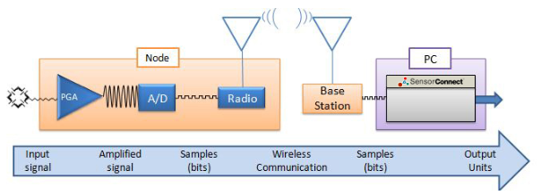
\includegraphics[width=1\textwidth, keepaspectratio]{lord_wireless.png}
        \caption[LORD drahtlose Übertragung (Abbildungsverzeichnis)]{LORD drahtlose Übertragung
        \cite{VLInkManual}
        }
        \label{fig:lordwireless}
    \end{center}
\end{figure}

Abbildung \ref{fig:lordwireless} zeigt die Funktionsweise der drahtlosen Datenübertragung.
Ein an den Node angeschlossener Sensor wird innerhalb des Nodes verstärkt und digitalisiert.
Anschließend werden die Messdaten vom Node drahtlos an eine Base Station gesendet welche mit einem Laptop verbunden ist.
Dort kann über die Software SensorConnect auf den Node zugegriffen werden und dessen Daten visualisiert oder weiterverarbeitet werden.


Abbildung \ref{fig:lordproducts} zeigt einen Teil der Produktpalette.
Als Gateway wurde von uns der dort gezeigte USB Stick genutzt.
Insgesamt wurden uns zwei VLINK 200 Node, und ein USB Stick zur Verfügung gestellt was in der späten Projektphase teilweise zu Problemen führte,
siehe \ref{sec:probleme} \nameref{sec:probleme}.

\begin{figure}[h]
    \begin{center}
        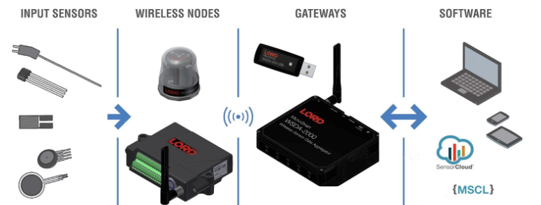
\includegraphics[width=1\textwidth, keepaspectratio]{lord_products.png}
        \caption[LORD Produkte (Abbildungsverzeichnis)]{LORD Produkte
        \cite{VLInkManual}
        }
        \label{fig:lordproducts}
    \end{center}
\end{figure}


\section{Dehnungsmessstreifen und Messprinzipien \(Bellgardt\)}
Dehnungsmessstreifen (DMS) sind sensorische Elemente, die zur Messung von mechanischen Dehnungen in Bauteilen eingesetzt werden. Das Wirkprinzip beruht auf der Änderung des elektrischen Widerstands eines metallischen oder halbleitenden Messgitters, wenn es durch eine mechanische Belastung gedehnt oder gestaucht wird. Diese Widerstandsänderung ist direkt proportional zur mechanischen Dehnung des Materials, auf das der DMS aufgeklebt ist. 
Das Messprinzip basiert auf dem Zusammenhang zwischen der mechanischen Dehnung und der Widerstandsänderung des DMS. Wird das Trägermaterial belastet, verändert sich seine Geometrie, wodurch sich auch die Länge und der Querschnitt des Messgitters ändern. Dies beschreibt die Gleichung des elektrischen Widerstands:

$R = \rho \cdot \frac{l}{A}$,

mit $\rho$ als spezifischem Widerstand, l als Länge und A als Querschnitt ergibt sich, dass eine Längenzunahme bei gleichzeitiger Verringerung des Querschnitts zu einer Erhöhung des Widerstands führt. Um diese Widerstandsänderung messbar zu machen, wird häufig eine Wheatstone-Brücke verwendet, die Spannungsänderungen proportional zur Dehnung des Materials erfasst.
DMS finden breite Anwendung in der experimentellen Spannungsanalyse, der Kraftmessung und der Strukturüberwachung in verschiedenen Ingenieurbereichen. Durch ihre hohe Empfindlichkeit und Präzision sind sie essenzielle Sensoren zur mechanischen Zustandsüberwachung von Bauteilen und Maschinen.










\newpage{}
\section{Viertel\-, Halb\- und Vollbr\"uckenschaltungen für DMS \(Bellgardt\)}
Zur präzisen Messung mechanischer Dehnungen werden Dehnungsmessstreifen häufig in Form einer Wheatstone-Brücke verschaltet. Dabei gibt es drei Hauptkonfigurationen: die Viertelbrücke, die Halbbrücke und die Vollbrücke, die sich in ihrer Empfindlichkeit, Temperaturkompensation und Messgenauigkeit unterscheiden.
\subsection{Viertelbrückenschaltung}
Die einfachste Form ist die Viertelbrückenschaltung (siehe Abbildung \ref{fig:fab1} links), bei der nur ein einzelner DMS als aktiver Widerstand in die Brückenschaltung integriert wird, während die anderen drei Widerstände passive Referenzwiderstände sind. Die Widerstandsänderung des DMS führt zu einer Veränderung der Brückenspannung, die als Messsignal ausgewertet wird. Da nur ein DMS aktiv zur Messung beiträgt, ist die Empfindlichkeit dieser Schaltung vergleichsweise gering. Zudem sind Temperaturkompensation und Störunterdrückung begrenzt, da äußere Einflüsse nicht ausreichend ausgeglichen werden. Die Viertelbrücke wird häufig in einfachen Spannungsmessungen eingesetzt, wenn nur geringe Genauigkeitsanforderungen bestehen.

\subsection{Halbbrückenschaltung}

Eine präzisere Alternative stellt die Halbbrückenschaltung  (siehe Abbildung \ref{fig:fab1} mittig) dar, bei der zwei DMS in die Brückenschaltung eingebaut sind. Diese werden oft so angeordnet, dass einer gedehnt und der andere gestaucht wird, wodurch sich ihre Widerstandsänderungen addieren und das Ausgangssignal verstärken. Dadurch erhöht sich die Messgenauigkeit im Vergleich zur Viertelbrücke. Gleichzeitig verbessert sich die Temperaturkompensation, da beide DMS denselben Umgebungseinflüssen ausgesetzt sind und sich temperaturbedingte Widerstandsänderungen teilweise gegenseitig aufheben. In diesem Projekt wurde hauptsächlich die Halbbrückenschaltung verwendet.

\subsection{Vollbrückenschaltung}
Die höchste Präzision und Empfindlichkeit bietet die Vollbrückenschaltung  (siehe Abbildung \ref{fig:fab1} rechts), bei der vier aktive DMS in die Wheatstone-Brücke integriert sind. Dabei befinden sich zwei DMS in einem gedehnten und zwei in einem gestauchten Zustand, wodurch sich ihre Widerstandsänderungen vollständig addieren und ein maximales Ausgangssignal erzeugt wird. Die Vollbrücke bietet nicht nur die beste Messgenauigkeit, sondern auch eine optimale Temperaturkompensation, da sich externe Temperatureinflüsse auf alle vier DMS gleichmäßig auswirken und somit weitgehend eliminiert werden.
Ein Vergleich dieser Brückenkonfigurationen findet sich zusammengefasst in Tabelle \ref{tbl:dms_schaltungen}.


\bgroup
\def\arraystretch{2}
\begin{table}[h]
\centering
\begin{tabular}{|p{0.25\linewidth}|p{0.25\linewidth}|p{0.25\linewidth}|p{0.25\linewidth}|}
\hline
Schaltung & Anzahl aktiver DMS & Empfindlichkeit & Anwendung \\ \hline
Viertelbrücke & 1 & Gering & Einfache Dehnungsmessung \\ \hline
Halbbrücke & 2 & Mittel & Biegung, Torsion, Kraftmessung \\ \hline
Vollbrücke & 4 & Hoch & Hochpräzise Messung, industrielle Sensorik \\ \hline
\end{tabular}
\caption{Vergleich verschiedener DMS-Schaltungen}
\label{tbl:dms_schaltungen}
\end{table}
\egroup


\begin{figure}[h]
    \begin{center}
        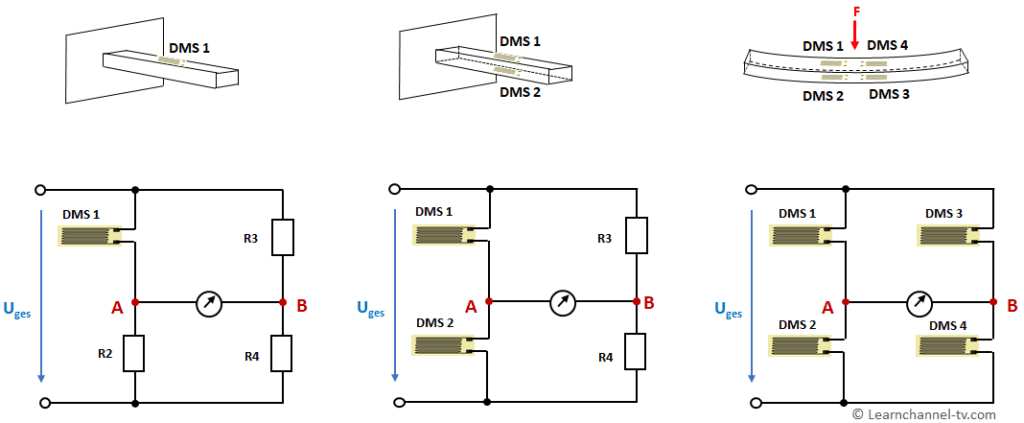
\includegraphics[width=1.0\textwidth, keepaspectratio]{fab1.png}
        \caption[DMS in Viertel\- Halb\- und Vollbr\"uckenkonfiguration (Abbildungsverzeichnis)]{DMS in Viertel\- Halb\- und Vollbr\"uckenkonfiguration
        \cite{LearnChannel}
        }
        \label{fig:fab1}
    \end{center}
\end{figure}






\section{Mechanische Belastungen \(Bellgardt\)}
Mechanische Belastungen entstehen, wenn äußere Kräfte oder Momente auf ein Bauteil einwirken und Spannungen sowie Verformungen im Material verursachen. Je nach Art der Beanspruchung unterscheidet man verschiedene Belastungsformen, die jeweils charakteristische Spannungs- und Dehnungszustände hervorrufen. Besonders relevant für die Dehnungsmessung sind Biegung, Torsion und axiale Kraftbeanspruchung, da sie mit Hilfe von Dehnungsmessstreifen (DMS) präzise erfasst werden können.

\begin{figure}[h]
    \begin{center}
        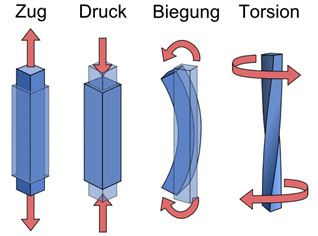
\includegraphics[width=0.5\textwidth, keepaspectratio]{fab2.png}
        \caption[Verschiedene Krafteinwirkungen (Abbildungsverzeichnis)]{Verschiedene Krafteinwirkungen
        \footcite{https://www.maschinenbau-wissen.de/bilder/skripte/mechanik/belastungsarten-03.PNG}
        }
        \label{fig:fab2}
    \end{center}
\end{figure}
\subsection{Biegung: Verformung durch einwirkende Kräfte}
Bei einer Biegebelastung wird ein Bauteil durch äußere Kräfte oder Momente gekrümmt. Dies führt zu einer Biegespannung, die entlang des Querschnitts eine typische Spannungsverteilung erzeugt: Auf der einen Seite des Bauteils tritt eine Dehnung (Zugspannung) auf, während die gegenüberliegende Seite gestaucht wird (Druckspannung). Dazwischen liegt die neutrale Faser, eine Linie oder Fläche ohne Längenänderung.
Zur Messung von Biegespannungen werden DMS typischerweise auf der Ober- und Unterseite des Bauteils angebracht. Eine Halbbrücken- oder Vollbrückenschaltung ist besonders vorteilhaft, da sie die Widerstandsänderungen der DMS kombiniert und sowohl die Empfindlichkeit als auch die Temperaturkompensation verbessert. Einsatzgebiete sind etwa: Bauwerksüberwachung, Maschinenbau und die Belastungsprüfung von Bauteilen.

\subsection{Torsion: Drehmomente und Schubspannungen}
Torsion tritt auf, wenn ein Bauteil um seine Längsachse verdreht wird, beispielsweise bei Antriebswellen oder Schraubverbindungen. Dabei entstehen Schubspannungen, die unter einem ±45°-Winkel zur Achse verlaufen.
Zur Messung von Torsionsbeanspruchungen werden DMS in einer schrägen Anordnung (meist in ±45°-Orientierung) angebracht, sodass sie die maximalen Schubspannungen erfassen. Eine Halbbrücke mit zwei DMS oder eine Vollbrücke mit vier DMS ermöglicht eine genaue Bestimmung des aufgebrachten Drehmoments. Eine Messung der Torsion wird oft für die Überwachung von rotierenden Maschinen, Fahrzeugantrieben und industriellen Wellen genutzt.

\subsection{Zug- und Druck}
Druck- und Zugkräfte treten auf, wenn äußere Kräfte entlang einer Achse auf ein Bauteil wirken und eine Längenänderung verursachen. Bei einer Zugbelastung wird das Bauteil gedehnt, während es bei einer Druckbelastung gestaucht wird. Diese mechanischen Dehnungen oder Stauchungen erzeugen Spannungen im Material, die mithilfe von Dehnungsmessstreifen (DMS) erfasst werden können.
Dies kann mit einem Kraftmesser gemessen werden.





\section{Biegebalken \(Menzel\)}
Die Entwicklung einer neuen Messtechnik für das Fahrrad und den Flying Suit stellt eine komplexe Aufgabe da.
Dies beinhaltet die Planung und Bestellung nötiger Materialien und die Anbringung dieser am jeweiligen Aufbau.
Um sicherzustellen, dass die zu entwickelnde technische Umsetzung möglich ist, wurde das Zusammenspiel von Node und Dehnungsmessstreifen zunächst am einfacheren Aufbau eines Biegebalkens getestet.


\subsection{Aufbau des Biegebalkens}
Auf der Ober- und Unterseite des Biegebalkens sind Dehnungsmessstreifen angebracht um die beim aufbringen eines Gewichts entstehende Dehnung messen zu können.
Dies wurde mit verschiedenen Gewichten und in verschiedenen Einheiten durchgeführt.
\begin{figure}[h]
    \begin{center}
        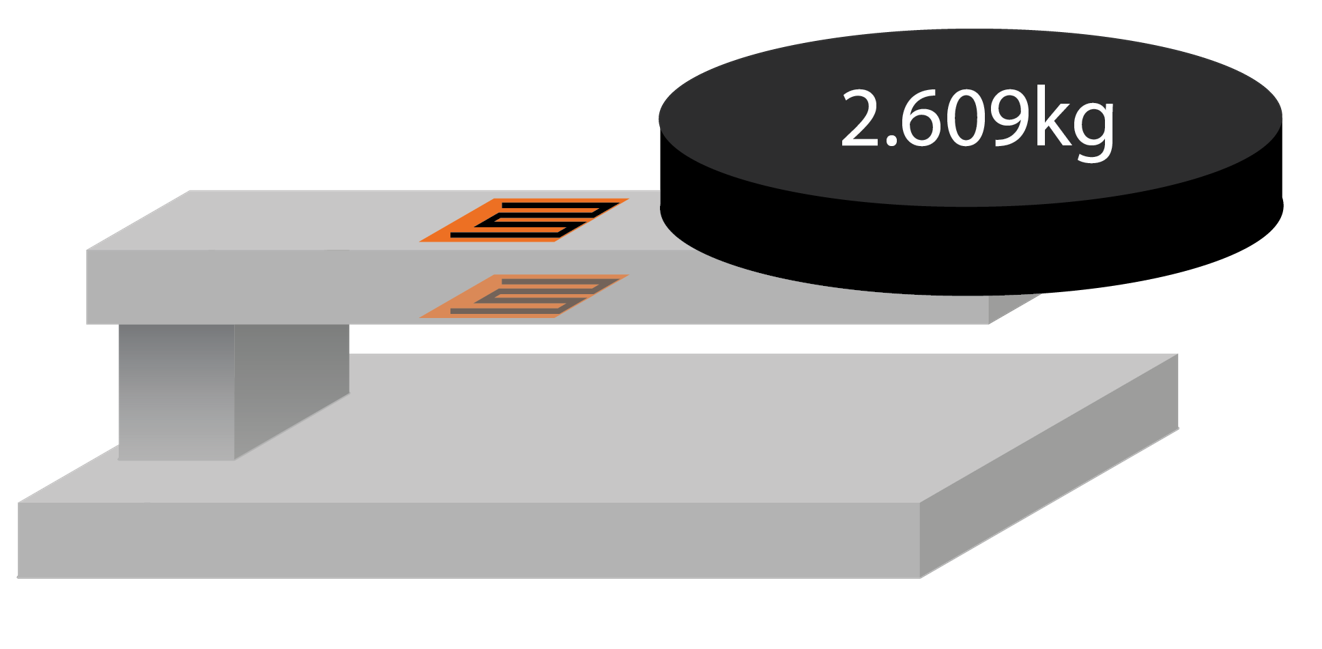
\includegraphics[width=0.5\textwidth, keepaspectratio]{biegebalken_grafik.png}
        \caption[Biegebalken Schema (Abbildungsverzeichnis)]{Biegebalken Schema
        %\cite{VLInkManual}
        }
        \label{fig:biegebalkenschema}
    \end{center}
\end{figure}

\subsection{Wahl des Messverfahrens}
Um Messungen durchführen zu können bieten sich verschiedene Verfahren an.
Die in der Software SensorConnect verfügbaren und für uns relevanten Verfahren sind die Shunt-, Field-, und Sensitivity(geometriebasierte)-kalibrierung.
Die Beschreibung sowie die Vor- und Nachteile dieser Verfahren sind in \ref{tbl:verfahren} \nameref{tbl:verfahren} dargestellt.
Um die theoretische Grundlage für den Aufbau des Fahrrads und des Flying Suits zu schaffen wurde sich beim Biegebalken für die Wahl des mV/V Messverfahrens entschieden.

\bgroup
\def\arraystretch{2}
\begin{table}[h]
\centering
\begin{tabular}{|p{0.25\linewidth}|p{0.25\linewidth}|p{0.25\linewidth}|p{0.25\linewidth}|}
\hline
Verfahren & Beschreibung & Vorteil & Nachteil\\ \hline
Shunt Kalibrierung & Interner (Shunt) Widerstand wird zur DMS-Brücke geschaltet. Es wird eine definierte Dehnung simuliert, um die Messkette zu überprüfen.
& schnell, einfach & Simuliert keine echte mech. Belastung, nur elektrische Effekte
\\ \hline
Field Kalibrierung & Messung von realer mech. Belastung mit Referenzlast

& Wenn Last bekannt ist, kann man sehr genau messen.
& Definierte Belastung der Struktur notwendig

\\ \hline
Geometriebasierte Kalibrierung (mV/V)
 & Berechnung für Software basierend auf Materialparametern und Geometrie


& Ermöglicht eine Abschätzung und Vergleich zwischen erwarteten und gemessenen Werten

& Abweichungen bei ungenauen Materialparametern möglich


\\ \hline

\end{tabular}
\caption{Messverfahren}
\label{tbl:verfahren}

\end{table}
\egroup


\subsection{Berechnung der Sensitivity}
Um eine Messung am Biegebalken durchführen zu können wurde zunächst die Sensitivity mathematisch berechnet.
Sie basierst auf der Geometrie des Biegebalkens, sowie des zu erwartendem maximalen Gewicht und wird als Parameter in SensorConnect eingegeben.
Sie stellt den gemessenen Wert in mV/V bei Maximalbelastung dar.
Aufgrund der einfachen Geometrie des Biegebalkens ist dies ein wichtiger Schritt, bevor diese für die komplexere Geometrie des Fahrradlenkers oder des Gestells des Flying Suits berechnet wird.

In der folgenden Berechnung wird für den Parameter n der Wert 2 verwendet, da es sich um die Anzahl der angebrachten DMS und die daraus resultierende Brückenkonfiguration handelt.
Der Parameter k ist durch die verwendeten DMS gegeben. Als maximale Last dient eine Hantelscheibe mit einem Gewicht von 2.609kg.



Maße des Biegebalkens:
\[
l = 117 \text{ mm}, \quad b = 19.8 \text{ mm}, \quad h = 2.94 \text{ mm}
\]
Maximale Last:
\[
M = 2.609 \text{ kg}
\]

\subsection*{Berechnung des Widerstandsmoments}
\[
W_x = \frac{b h^2}{6}
\]
Einsetzen der Werte:
\[
W_x = \frac{19.8 \times 2.94^2}{6} = 28.52 \text{ mm}^3
\]

\subsection*{Berechnung des Biegemoments}
\[
M_b = F \times l
\]
\[
M_b = 2.609 \times 9.81 \times 117mm = 2994.53 \text{ Nmm}
\]

\subsection*{Berechnung der Spannung}
\[
\sigma = \frac{M_b}{W_x}
\]
\[
\sigma = \frac{2994.53}{28.52} = 104.99 \text{ N/mm}^2
\]

\subsection*{Berechnung der Dehnung}
\[
\varepsilon = \frac{\sigma}{E}
\]
Mit \(E = 210000 \text{ N/mm}^2\):
\[
\varepsilon = \frac{104.99}{210000} = 0.499\times 10^{-3}
\]

\subsection*{Berechnung der Brückenausgabe}
\[
\frac{U_M}{U_B} = \frac{n}{4} \times k \times \varepsilon
\]
Mit \( n = 2 \), \( k = 2.01 \):
\[
\frac{U_M}{U_B} = \frac{2}{4} \times 2.01 \times 0.499 \times 10^{-3}
\]
\[
\frac{U_M}{U_B} = 0.000502 \text{ V/V} = 0.5 \text{ mV/V}
\]

Mit der berechneten Sensitivity wurden mehrere Messungen durchgeführt.
Die erste Messung wurde mit einem Gewicht von 2.609kg durchgeführt und in MPa gemessen, siehe \ref{tbl:biegebalkenmessungeins} \nameref{tbl:biegebalkenmessungeins}.

\bgroup
\def\arraystretch{2}
\begin{table}[h]
\centering
\begin{tabular}{|p{0.33\linewidth}|p{0.33\linewidth}|p{0.33\linewidth}|}
\hline
Gegeben & Gemessen & Abweichung \\ \hline
105MPa (2.609kg) & 120MPa (2.8kg) & +14\% \\ \hline
\end{tabular}
\caption{Messung 1 mit Maximalgewicht, [MPa]}
\label{tbl:biegebalkenmessungeins}

\end{table}
\egroup

Die zweite Messung wurde mit verschiedenen Gewichten getestet und in N gemessen, siehe \ref{tbl:biegebalkenmessungzwei} \nameref{tbl:biegebalkenmessungzwei}.
\bgroup
\def\arraystretch{2}
\begin{table}[h]
\centering
\begin{tabular}{|p{0.33\linewidth}|p{0.33\linewidth}|p{0.33\linewidth}|}
\hline
Gegeben & Gemessen & Abweichung \\ \hline
0N (0kg) & 0.2N (0.02kg) & - \\ \hline
3.9N (0.4kg) & 4.6N (0.46kg) & +17.9\%  \\ \hline
24.5N (2.609kg) & 27.6N (2.81kg)  & +12.6\% \\ \hline
\end{tabular}
\caption{Messung 2, [N]}
\label{tbl:biegebalkenmessungzwei}

\end{table}
\egroup

